%!TEX encoding = UTF-8 Unicode
%!TEX program = xelatex

\documentclass[master,pagecenter]{ustcthesis}
% bachelor|master|doctor
\usepackage{ustcextra}
\graphicspath{{figures/}}
% \bibliographystyle{ustcauthorybbear}
\bibliographystyle{ustcnumerical}
\citestyle{ustcnumerical}
\title{老年猕猴视皮层细胞 \texorpdfstring{\\ 的功能衰退}{}}
\author{柴泉}
\major{软件工程}
\advisor{孙建伶\ 教授}
\coadvisor{刘耀庭\ 教授}
\submitdate{二〇一六年八月七日}
%\secrettext{机密\quad 小于等于20年}   % 内部|秘密|机密,注释本行则不保密
% \depart{一二三系}

\entitle{The Function Degradation in Visual Cortical Cells of old rhesus Monkeys}
\enauthor{Chai Quan}
\enmajor{Software Engineering}
\enadvisor{Prof. JianLin Sun}
\encoadvisor{Prof. YaoTing Liu}
\ensubmitdate{August 7th, 2016}
%\ensecrettext{Confidential\quad Less than or equal to 20 years}  % Internal|Secret|Confidential

\begin{document}
\maketitle

%
% 本科论文:
%   frontmatter: 致谢、目录、中文摘要、英文摘要
%   mainmatter: 正文章节、参考文献
%   appendix: 附录
%
% 硕博论文:
%   frontmatter: 中文摘要、英文摘要、目录、符号说明
%   mainmatter: 正文、参考文献
%   appendix: 附录
%   backmatter: 致谢、发表论文
%

\frontmatter{}
\begin{abstract}
衰老使得正常的视觉功能受到严重影响,眼睛光学系统的老年性改变并不足以解释这种视觉功能衰退,一般认为是神经系统的退化导致了这种老年性功能降低。过去几年中在老年动物视觉皮层发现了一系列细胞反应特性的改变,这些细胞水平的变化被认为是老年性视觉功能衰退的神经机制。为了更全面的了解衰老过程对视觉皮层的影响以及细胞反应改变与整体功能降低之间的关系,本研究采用在体细胞单位外单位记录方法,从以下三个方面进一步比较了青年和老年猕猴视觉皮层细胞反应特性的差异:

以前的研究发现在老年猕猴初级视皮层(V1),细胞正常的反应特性发生了与功能退化相关的改变。为了研究这种细胞反应特性的改变如何在皮层视觉通路中传递,本实验研究了衰老对猕猴次级视皮层(V2)细胞功能的影响。我们发现,与年轻猴相比,老年猕猴V2细胞的方位、方向选择性明显下降,同时自发放电活动增加,视觉刺激诱发的反应幅度增加以及细胞活动的信噪比降低。由于V2区在复杂视觉信息处理过程中有重要作用,本结果提供了衰老影响较高级视觉功能可能的神经机制。与V1区细胞的老年性功能退化相比较,V2区细胞反应特性受老化的影响更为严重。与V1区细胞的老年性功能退化相比较,V2区细胞反应特性受老化的影响更为严重,这说明V2区表现出的功能退化并非完全由V1区的变化引起,衰老的影响可能在皮层视觉通路中逐渐积累。

通过上述三个实验,我们研究了灵长类动物视皮层细胞老年性功能退化在不同脑区的表现特点,随衰老而变化的动态过程以及细胞信息处理能力所受衰老的影响。这些结果更加完整的描述了老年性视觉功能下降的神经机制。

论文摘要可以以列表的形式列出自己的主要工作:
\begin{enumerate}
\item 本论文提出了XXX的解决方案。
\item 本论文使用XXX技术进行实现。
\item 本论文基于XXX。
\end{enumerate}

\keywords{衰老,功能退化,初级视皮层,次级视皮层,兴奋-抑制平衡,信息处理,猕猴}
\end{abstract}

\begin{enabstract}
Visual function is influenced significantly by aging. The aging-related visual deficits can be observed even after the optical factor has been well controlled, suggesting the important role the central nerve system played in generation of such deficits. In the past few years, several alterations in response properties of visual cortical cells have been reported in senescent animal models, which were considered as the neural mechanisms underlying the aging-related degradation of vision. In order to get a more comprehensive understanding about the aging effects on visual cortices and the relationship between the changes at cellular level and the functional degeneration at the whole system level, in the present study, we used in vivo extracellular single-unit recording techniques to compare the response property of visual cortical eclls in young and old monkeys. The study included three experiments:

By these three experiments, we studied the different characteristics of aging effects in different brain areas, the dynamics of these effects and the impairments of signal processing during senescence. All of these findings provided us a more comprehensive understanding about the mechanisms underlying the aging-related degeneration of visual function.


\enkeywords{aging, function degeneration, primary visual, secondary visual cortex, balance between excitation and inhibition, signal processing, rhesus monkey}
\end{enabstract}

\tableofcontents
\listoffigures
\listoftables
% \listofalgorithms  % 算法索引,如不需要,可直接注释掉本行
% \input{chapters/notation}

\mainmatter
\chapter{绪论}
\section{研究背景}

次级视皮层(V2)是皮层视觉通路上的第二个环节,从初级视皮层(V1)传出的信息,大部分经过V2送到其他纹状外视觉皮层。除了V1区的传入外,V2还接受丘脑枕核(pulvinar)的信息以及其他纹状外视觉皮层(包括背侧和腹侧的视觉通路)的反馈。所以,作为一个信息整合与反馈控制的枢纽,V2是视觉信息传递与处理过程中的重要一站\cite{01}。

此段是介绍论文的研究背景,建议写1.5页。并有3到5个左右的引用。



\section{国内外研究现状}
\subsection{XXX概述}


这一节,针对论文中设计的技术进行一个简要的发展历史说明。


\subsection{XXX介绍}

针对论文中使用的专业技术进行详尽的介绍。

\section{本论文的主要工作}

在论文绪论中介绍自己的主要工作,最好使用列表的形式。
根据上述研究内容和研究目标,本文主要的工作从以下几个方面展开:
\begin{enumerate}
\item 实现了一个XXX的模拟方案,在此基础上进行了相应的改进。
\item 由于XXX的局限性,从而提出了基于XXXX保存方法。
\item 采用XXX技术实现复杂的YYY。
\item 基于以上的理论研究和技术调研,实现了一个XXX。
\end{enumerate}
\section{本论文的组织结构}
本文主要分为七个章节,每个章节的具体内容安排如下:
\begin{enumerate}
\item 绪论:介绍XXX技术的发展,以及早期YYY的各种不足,XXX的出现和所解决的问题。
\item XXX的相关知识:介绍了使用XXX技术开发YYY所需要的相关知识。主要包括ZZZ方程的介绍、XXX技术的基本概念、YYY的坐标变化和XXX。
\item 需求分析:通过对XXX的调研,得出本系统开发和研究的必要性。
\item 概要设计:基于需求分析的基础,提出应用XXX技术合适的设计方案,包括XYZ。通过概要设计,为整个系统的实现做好铺垫。
\item 详细设计与实现:基于概要分析的设计方案,使用XXX技术去实现烟雾模拟系统。这部分主要是讲述每个设计过程中涉及的实现细节,通过对开发过程中难点的攻克,得以最终实现了一个XXX系统。
\item 系统测试与分析:在实现XXX系统之后,我们要对整个系统进行测评,主要是从功能性、稳定性、性能和视觉效果四个方面来分析,确保最终表现的渲染效果满足预期的结果。
\item 总结与展望:总结自己本文所完成的工作,以及对于XXX的未来发展的展望,并指出自己当前研究的不足之处有待日后改进。
\end{enumerate}

% 以下的代码确保余下的章节不会都在右边开始,导致左边的页面留白


\makeatletter
\@openrightfalse
\makeatother
\chapter{XXX以及YYY的相关知识}
\section{Navier-Stokes方程}

本章的主要内容是介绍论文使用的相关技术,篇幅不易过多。

上述假设是使用N-S方程必须满足的条件,通常N-S方程需要用下面的方程式来描述\cite{02}:

\begin{equation} \label{eq:1}
\frac{\partial \vec u}{\partial t} = - \vec u \cdot \nabla \vec u - \frac{1}{\rho}\nabla p +\nu \nabla \cdot \nabla \vec u  + F
\end{equation}
\begin{equation} \label{eq:2}
\nabla \cdot \vec u = 0
\end{equation}

其中,$\vec{u}$用来表示流体运动的速度场,${t}$代表时间。希腊字母$\rho$代表流体的密度,对于水来说通常是$1000kg/m^{3}$,对于空气来说通常是$1.3kg/m^{3}$。$p$ 代表压力,是施加在流体上的单位面积上的力。希腊字母$\nu$ 为运动粘性系数(kinematic viscosity),又称为动量扩散率,粘度通常表示一种阻碍物体流动的属性,不同的流体具有不同的粘度,例如糖浆具有高粘度,而酒精具有低粘度。$F$指得是作用在流体上的任何外力\cite{03}。方程(\ref{eq:1})是流体的动量守恒方程,方程(\ref{eq:2})是流体的不可压缩方程。

符号$\nabla$称为微分运算符(nabla operator),主要应用在梯度(gradient)、散度(divergence)、普拉斯算子(Laplacian operators)中,如表\ref{tab:1}所示。

\renewcommand\arraystretch{2.5}
\begin{table}[htbp]
\centering
\caption{微分运算符在XXX中的应用} \label{tab:1}
\begin{tabular}{|l|c|c|}

    \hline
    操作 & 定义 & 有限微分形式 \\
    \hline
    梯度 & $ \displaystyle \nabla p = \Bigl( \frac{\partial p}{\partial x} , \frac{\partial p}{\partial y} \Bigr)$ & $\displaystyle \frac{p_{i+1,j} - p_{i-1,j}}{2\delta x} , \frac{p_{i,j+1} - p_{i,j-1}}{2\delta y}$ \\
    \hline
    散度 & $ \displaystyle \nabla \cdot u  =  \frac{\partial u}{\partial x} + \frac{\partial v}{\partial y} $ & $ \displaystyle \frac{u_{i+1,j} - u_{i-1,j}}{2\delta x} + \frac{v_{i,j+1} - v_{i,j-1}}{2\delta y}$ \\
    \hline
    普拉斯算子 & $ \displaystyle \nabla^2 p =  \frac{\partial^2 p}{\partial x^2} + \frac{\partial^2 p}{\partial y^2}$ & $ \displaystyle \frac{p_{i+1,j}  - 2p_{i,j} + p_{i-1,j}}{(\delta x)^2} + \frac{p_{i,j+1}  - 2p_{i,j} + p_{i,j-1}}{(\delta y)^2}$ \\
    \hline
\end{tabular}
\end{table}

梯度,标量场的梯度是一个向量场。散度,出现在方程(\ref{eq:2}),是求解N-S方程的关键,通过流体的不可压缩方程我们知道每个时间片结束的时候速度的散度为0。散度是向量场的一种强度性质,散度描述的是向量场里一个点是汇聚点还是发散点。普拉斯算子实际上就是$\delta^2 = \delta \cdot \delta$,定义为梯度的散度。

对于方程(\ref{eq:1}),从左到右依次是,平流项($- \vec u \cdot \nabla \vec u$),压力项($- \frac{1}{\rho}\nabla p$),扩散项($\nu \nabla \cdot \nabla \vec u$)和外力项($F$)。接下来介绍这四项的含义\cite{04}:
\begin{enumerate}
\item 平流项:流体的平流项指的是流体沿着自身速度的方向传递物体、密度或其他量。例如把墨水倒入流动的液体中,墨水会沿着液体的速度场进行传送。并且,流体的速度也携带流体自身。因此方程(\ref{eq:1})中的$- \vec u \cdot \nabla \vec u$表示速度场本身的平流,被称为平流项。
\item 压力项:因为流体中的分子可以相互运动,所以分子之间会产生``挤压''和``碰撞''。当外力作用到流体上的时候,它并不会直接传导到整个流体空间,而是通过分子之间的相互作用,离外力近的分子把那些离外力远的分子推开,这样压力就慢慢作用到整个流体上。因为压力是单位面积上的力,流体中的任何压力都会产生加速度。方程的第二项成为压力项,就是代表这个加速度。
\item 扩散项:通过日常情境下对流体的观察可以发现,每一种流体都有着不一样的粘度。例如,蜂蜜的流动就比酒精要慢很多,一般越浓稠的液体粘度越高。粘度一般指在流体运动中所受到的阻力影响,从而导致动量的四处扩散,因此引起了速度的扩散,所以第三项是扩散项。
\item 外力项:外力指的是流体受到外力作用产生的加速度。外力可以是局部的,也可以是整体的。例如重力和浮力都是针对整个流体施加的,而电吹风只能施加到流体的一部分,是属于局部力的范畴。
\end{enumerate}

我留了一个方程和图表供大家参考,如何正确的使用Latex书写方程和表格,希望大家都喜欢上这种书写方式。


\section{本章小结}

除了绪论,每章的最后一节都必须有本章小结,这是学校的规定。

\chapter{需求分析}
\section{选题的动机与目的}

介绍下为什么选择这个论文课题以及好处和优势。

我们选用XXX技术来开发的原因主要有以下两点:

\begin{enumerate}
\item 简化了开发成本:一次开发,多平台使用。和传统的客户端开发模式不同,XXX技术的跨平台性使得我们不需要针对特定的平台而进行额外的开发工作,用户只需要安装通用的浏览器即可正常使用。
\item 节约了系统的维护:因为我们所有的项目文件都是保存在服务器上,用户每次加载资源都需要从服务器上重新下载,所以在后期维护和更新项目的过程中,不再需要用户进行参与,直接通过服务器上的更新就可以很方便的完成升级和快速迭代开发。
\end{enumerate}

\section{选题的可行性分析}

经过本人的调研和研究,XXX技术通过完全可以胜任在YYY中实现复杂的ZZZ,并获得良好的实时效果,足以达到最终的需求。

\subsection{主要技术路线}
\begin{itemize}
  \item 应用架构:B/S架构
  \item 前台技术:HTML5
  \item 3D展现层:XXX
  \item 算法基础:Navier-Stokes方程
\end{itemize}

\subsection{核心技术关键}
\begin{itemize}
  \item 三维数据的操作与保存
  \item 求解Navier-Stokes方程
\end{itemize}

\section{本系统的需求概述}

一段话对当前的需求进行描述。

\section{本系统的功能性需求描述}

针对本论文实现的系统的具体功能点来列出每个功能的需求,最好使用用例图来进行描述。

\section{本系统的非功能性需求描述}

本系统的非功能性需求主要有以下四个方面:
\begin{enumerate}
\item 系统运行的效率
\item 系统运行的稳定性
\item 系统的可扩展性
\item 系统运行的真实性
\end{enumerate}
\section{本章小结}

除了绪论,每章的最后一节都必须有本章小结,这是学校的规定。
\chapter{概要设计}

概要设计主要是讲述系统的架构设计和提出的一些解决方案。概要设计及以后的章节都尽量不要出现引用内容,因为已经属于自己的研究成果部分了。

\section{系统架构}

由需求分析可知,本系统总共有两个模块,首先是求解N-S方程模块,针对N-S方程的每个部分展开分别求解,其次是WebGL渲染模块,主要设计的是流程控制和最后的烟雾运动渲染。本系统的软件结构如图\ref{fig:struct}所示。

\begin{figure}[ht]
\centering
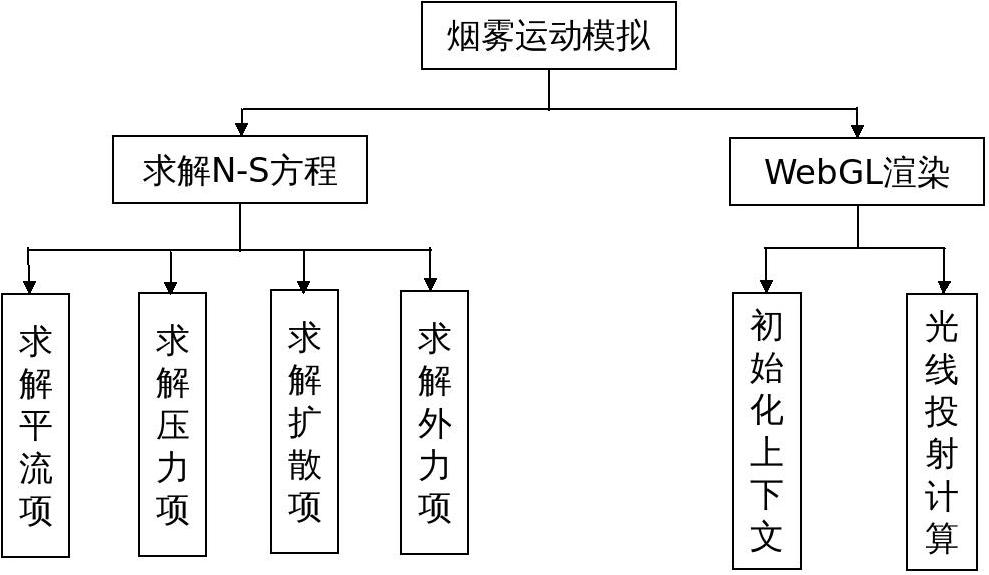
\includegraphics[width=300pt]{struct.jpeg}
\caption{本系统结构图} \label{fig:struct}
\end{figure}

各个模块的主要职责如下:

\begin{itemize}
  \item N-S方程求解模块:主要负责XXX。
  \item WebGL控制模块:主要负责YYY。
\end{itemize}

概要设计的第一个小标题应该是整个论文设计系统的架构,并附上结构图。

\section{本章小结}

除了绪论,每章的最后一节都必须有本章小结,这是学校的规定。
\chapter{详细设计与实现}

详细设计是根据概要设计的基础,对每个模块进行详尽的介绍和讲述具体的实现细节。

此章可以多使用流程图,数据流图等软件工程的方式来描述具体的实现细节。尽快不要贴代码。

\section{本章小结}

除了绪论,每章的最后一节都必须有本章小结,这是学校的规定。
\chapter{系统测试与分析}

在实现完之后,要通过详尽的测试来保证系统的健全。

\section{测试平台的搭建}

本文对烟雾运动模拟系统进行了详细的测试,测试的环境为:

\begin{itemize}
  \item 硬件平台:Intel Core i7-4790处理器,32GB内存,NVIDIA GeForce GTX 860独立显卡,2GB显存。
  \item 软件平台:Windows 10 64bit操作系统,Chrome 55 浏览器,Sublime Text文本编辑器。
\end{itemize}


\section{测试的目的}

对软件系统的测试,是软件开发周期的最后一道工序也是软件质量的保证。我们应该在测试的过程中尽量发现软件的缺陷并进行修补。在不同的开发阶段修补缺陷的成本是不一样的,软件BUG发现的越晚,特别是在软件发布之后,我们为修补BUG所付出的代价就越大,有时还会影响用户体验。因此对软件进行测试是保证软件质量的有效手段,我们应当在发布系统之前进行详尽的测试,测试达到的主要目标有:

\begin{enumerate}
\item 系统的功能性
\item 系统的运行性能
\item 系统的稳定性
\item 系统的视觉效果
\end{enumerate}


\section{系统的功能性测试}

针对需求分析里提出的功能点,逐一进行测试。

\section{系统的稳定性测试}

测试系统在各种边界条件下的稳定性,保证运行不会崩溃或有内存泄漏等意外情况发生。

\section{系统的运行性能测试}


针对系统的运行性能和效率进行测试,可以采用各种测试工具来形象的说明测试结果。


\section{系统的视觉效果测试}

这是针对图形学论文的特殊测试,其他项目可以不需要这个子标题。

\section{本章小结}

除了绪论,每章的最后一节都必须有本章小结,这是学校的规定。
\chapter{总结与展望}
\section{论文工作总结}

列大纲介绍下自己的主要工作。
 

\section{论文未来展望}


论文的未来研究方向。

本文有待改进的工作: 
使用列表列出不足和需要改进的地方。

% 以下的代码确保每个页面都在右边打开


\makeatletter
\@openrighttrue
\makeatother
\begin{thebibliography}{35}

\bibitem{01} Alexey Demin,代沅兴,李新等.基于HTML5与WebGL的机器人3D环境下的运动学仿真[J].东北大学学报(自然科学版),2014,35(4):564-568.
\bibitem{02} 韩义.Web3D及Web三维可视化新发展——以WebGL和03D为例[J].科技广场,2010,(5):81-86.
\bibitem{03} Marrin, Chris. Webgl specification[J]. Khronos WebGL Working Group (2011).
\bibitem{04} 李伟伟. 在GPU上实现的基于物理的流体模拟[D].吉林大学,2009.

\end{thebibliography}

\appendix


\backmatter
\begin{acknowledgements}

总是在快要结束的时候才会发现,校园时光走得太快,从来不会因为留恋而停下脚步。转瞬之间两年半的硕士研究生学习生涯即将结束。在中科大攻读研究生期间,得到了太多人的关怀,有同学的帮助,老师的指导,父母的关爱,当然也少不了自己不敢居人后的努力。论文的撰写是一个非常艰苦的过程,在那些苦苦思索的夜晚,在踌躇的编写过程当中,我不仅对自己的专业知识有了更深刻的巩固,更学会了如何把自己的所学所知和研究内容有条不紊的表达出来。

在这里,我要感谢软件学院的全体师生,为我们提供良好的学习环境,更要特别感谢我的导师孙建伶教授,不仅给予我悉心的指导,并不辞辛苦的帮助我完善论文。

同时,我还要感谢我的企业导师刘耀庭教授,在学习上和生活上都给予了我各种帮助,让我得以顺利完成论文,其中教授的人格和学识为我留下了深刻的印象。

另外,我必须要对我的父母致以亲切的感谢。是他们在背后默默的为我提供了良好的学习环境和经济支持,从小到大,父母给了我太多包容和无条件的支持,让我能够心无旁骛的在知识的海洋中畅游。他们是一群最为普通的人,在我心中却最为伟大,如果没有父母的无言却有力的支撑,我是不会一路走到这里的。真的特别感谢他们!

最后,我还要感谢研究生期间陪伴在我身边的同学、朋友,感谢他们给我提出宝贵的建议和专业的见解,正是有了他们的支持和鼓励,我才能度过一段美好且充实的学习生涯。

最后,对百忙之中抽出时间审阅本论文的专家学者,表示由衷的感谢!

\end{acknowledgements}


\begin{advice}

非常感谢两位盲审导师和答辩委员会在百忙之中审阅我的论文,并给出中肯的修改建议,本人已综合各位老师的修改建议,并根据具体内容逐一修改,以下是论文的修改说明。

\begin{enumerate}
\item 对论文的文字和图进行调整,如图 6.1 未被引用,即需要检查全文的图表,确保每个图表都能被正确引用。 
\item 英文摘要存在多处不通顺词:重新书写英文摘要,并着重检查语法问题。
\item 图不清晰如图5.3,实验中表中的数据没有分析如表6.1:更新图5.3使表达更清晰,对表6.1在下方的文字描述中详细描述失败情况,并作出解释。
\end{enumerate}

\end{advice}


% \begin{publications}

\section*{已发表论文}

\begin{enumerate}
\item A A A A A A A A A
\item A A A A A A A A A
\item A A A A A A A A A
\end{enumerate}

\section*{待发表论文}

\begin{enumerate}
\item A A A A A A A A A
\item A A A A A A A A A
\item A A A A A A A A A
\end{enumerate}

\section*{研究报告}
\begin{enumerate}
\item A A A A A A A A A
\item A A A A A A A A A
\item A A A A A A A A A
\end{enumerate}

\end{publications}


\end{document}
